\section{Controllable Generation}

%\begin{frame}
%\subsectionpage
%\end{frame}

\begin{frame}{Controllable Generation}
\begin{center}
\resizebox{0.7\textwidth}{!}{
\begin{tikzpicture}

    \node[anchor=west] (mr) at (0.5,-2.8) 
       {\resizebox{5.5cm}{!}{$\pi\left( \left[\!\!\!\left[ \begin{array}{l}
        \textsc{Inform}\\
        \textrm{\color{Red}name=Aromi}\\
        \textrm{\color{Green}eat\_type=coffee shop}\\
        \textrm{\color{Blue}area=city centre}\\
    \end{array}\right]\!\!\!\right]\right)$ }};

\node[draw] (gen) at ($(mr.east)+(2,0)$) {NLG Model};

\node[draw,anchor=west,text width=5cm] (u2) at ($(gen.east)+(2,0)$) {\textit{{\color{Red}Aromi} is located in the {\color{Blue}city centre} and serves {\color{Green}coffee}.}};

\node[draw,anchor=south west,text width=5cm] (u1) at ($(u2.north west)+(0,1)$) {\textit{For {\color{Green}coffee} in the {\color{Blue}city centre}, try {\color{Red}Aromi}.}};
\node[draw,anchor=north west,text width=5cm] (u3) at ($(u2.south west)+(0,-1)$) {\textit{If you are in the {\color{Blue}city centre}, try {\color{Red}Aromi} for {\color{Green}coffee}.}};


\draw[line width=0.5mm,->] (mr) -- (gen.west);
\draw[line width=0.5mm,->] (gen.east) -- (u1.west);
\draw[line width=0.5mm,->] (gen.east) -- (u2.west);
\draw[line width=0.5mm,->] (gen.east) -- (u3.west);

\node[text=black,fill=white,draw=white] at ($(gen.east)!0.5!(u1.west)$) {\large ?};
\node[text=black,fill=white,draw=white] at ($(gen.east)!0.5!(u2.west)$) {\large ?};
\node[text=black,fill=white,draw=white] at ($(gen.east)!0.5!(u3.west)$) {\large ?};




\end{tikzpicture}}
\end{center}

\begin{itemize}
\item Realization order of neural NLG models is determined implicitly by the decoder
language model. 
\item Not possible to specifiy an ordering of the attribute-values
\textit{a priori} when generating.

\item Control is desirable for summarization, especially if we want to be able
to add more organization to longer summaries or implement discourse ordering
strategies.

\end{itemize}

\end{frame}



\begin{frame}{Alignment Training Yields Controllable Generation}

\begin{itemize}
    \item Alignment Training, an input transformation for Seq2Seq to models,
    makes a model controllable at the level of
    realization ordering.

\end{itemize}
\end{frame}

%\subsection{Alignment Training}
%
%\begin{frame}
%\subsectionpage
%\end{frame}

\begin{frame}{Alignment Training}
   
    \begin{center}
    \resizebox{0.65\textwidth}{!}{
    \begin{tikzpicture}
   \draw[mLightBrown!30] (6.2,0) -- (6.2,-8.15);
%   \uncover<4-5>{
%   \draw[mLightBrown!30] (6.2,0) -- (6.2,-9.21);
%   }
   \draw[mLightBrown!30] (0,0) -- (0,-4.85);

   \uncover<1-3>{
       \node[align=left,text width=10cm,anchor=north west] at (0,0) {\texttt{{\color{mLightBrown}\# Input}\\x = [\\~\\~\\~\\~\\~\\~\\]}};
   }
   \uncover<1-2>{
       \node[anchor=west] at (0.5,-2.8) 
       {\resizebox{5.5cm}{!}{$\pi\left( \left[\!\!\!\left[ \begin{array}{l}
        \textsc{Inform}\\
        \textrm{\only<2>{\color{Red}}name=Aromi}\\
        \textrm{\only<2>{\color{Green}}eat\_type=coffee shop}\\
        \textrm{\only<2>{\color{Blue}}area=city centre}\\
    \end{array}\right]\!\!\!\right]\right)$ }};


   }
\uncover<2>{
    \draw[line width=1.5mm,draw=Green,<->] (5.4,-3.1) to [out=0,in=270] (6.15,-2.8) to [out=90,in=180] (6.8,-2.5);
\node at (4.25,-2.55) {};
    \draw[line width=1.5mm,draw=Red,<->] (4.20,-2.55) to [out=0,in=90] (6.15,-3.10) to [out=270,in=180] (6.70,-6.36);
    \draw[line width=1.5mm,draw=Blue,<->] (4.70,-3.56) to [out=0,in=180] (6.70,-4.36);
}
\uncover<3>{
    \draw[line width=1.5mm,draw=Green,<->] (5.2,-2.5) to [out=0,in=180] (6.8,-2.5);
\node at (4.25,-2.55) {};
    \draw[line width=1.5mm,draw=Red,<->] (3.20,-3.55) to [out=0,in=180] (6.70,-6.36);
    \draw[line width=1.5mm,draw=Blue,<->] (4.40,-3.0) to [out=0,in=180] (6.70,-4.36);
}
%%\uncover<5>{
%    \draw[line width=1.5mm,draw=Green,<->] (5.2,-2.5) to [out=0,in=180] (6.8,-3.7);
%\node at (4.25,-2.55) {};
%    \draw[line width=1.5mm,draw=Red,<->] (3.20,-3.00) to [out=0,in=90] (5.85,-4.08) to [out=270,in=180] (6.70,-5.16);
%    \draw[line width=1.5mm,draw=Blue,<->] (4.40,-3.55) to [out=0,in=180] (6.70,-7.06);
%}

   \uncover<3>{
       \node[align=left,text width=10cm,anchor=north west] at (0,0) {\texttt{{\color{mLightBrown}\# Input}\\x = [\\
                    ~~~~"<<s>>",\\
                ~~~~"inform",\\
                ~~~~{\color{Green}"eat\_type=coffee shop",}\\
                ~~~~{\color{Blue}"area=city centre",}\\
                ~~~~{\color{Red}"name=Aromi",}\\
                ~~~~"<<e>>"\\
            ]\\~
   }};
}
%   \uncover<5>{
%       \node[align=left,text width=10cm,anchor=north west] at (0,0) {\texttt{{\color{mLightBrown}\# Input}\\x = [\\
%                    ~~~~"<<s>>",\\
%                ~~~~"inform",\\
%                ~~~~{\color{Green}"eat\_type=coffee shop",}\\
%                ~~~~{\color{Red}"name=Aromi",}\\
%                ~~~~{\color{Blue}"area=city centre",}\\
%                ~~~~"<<e>>"\\
%            ]\\~
%   }};
%}
   \uncover<1-3>{
         \node[align=left,text width=3cm,anchor=north west] at (6.2,0) {\texttt{{\color{mLightBrown}\# Output}\\y = [\\ 
                    ~~~~"<<s>>",\\ 
                    ~~~~"for",\\
                    ~~~~\only<1>{"coffee",}\only<2->{{\color{Green}"coffee",}}\\
                    ~~~~"in",\\
                    ~~~~"the",\\
                ~~~~{\only<2->{\color{Blue}}"city",}\\
            ~~~~{\only<2->{\color{Blue}}"centre",}\\
                    ~~~~",",\\
                    ~~~~"try",\\
                ~~~~{\only<2->{\color{Red}}"aromi",}\\
                    ~~~~".",\\
                    ~~~~"<<e>>"\\
                ] \\ ~
   }};
   }

%   \uncover<4-5>{
%         \node[align=left,text width=5.75cm,anchor=north west] at (6.2,0) {\texttt{{\color{mLightBrown}\# Output}\\y = [\\ 
%                    ~~~~"<<s>>",\\ 
%                    ~~~~"there",\\
%                    ~~~~"is",\\
%                    ~~~~"a",\\
%                    ~~~~{{\color{Green}"coffee",}}\\
%                    ~~~~{{\color{Green}"shop",}}\\
%                    ~~~~"called",\\
%                ~~~~{\color{Red}"aromi",}\\
%                    ~~~~"in",\\
%                    ~~~~"the",\\
%                ~~~~{\color{Blue}"city",}\\
%            ~~~~{\color{Blue}"centre",}\\
%                    ~~~~".",\\
%                    ~~~~"<<e>>"\\
%                ] \\ ~
%   }};
%   }


   \uncover<2->{
   \node[text width=5cm,anchor=north west] at (0,-5) {\begin{enumerate} \item Align utterance \texttt{y} to attribute-values. \item<3-> Order \texttt{x} according to the order the attribute-values are realized in \texttt{y}.\end{enumerate}};
   }
    \end{tikzpicture}
}
\end{center}
\end{frame}

\begin{frame}{Alignment Training Yields Controllable Generation}
  \begin{center}
    \resizebox{0.70\textwidth}{!}{
    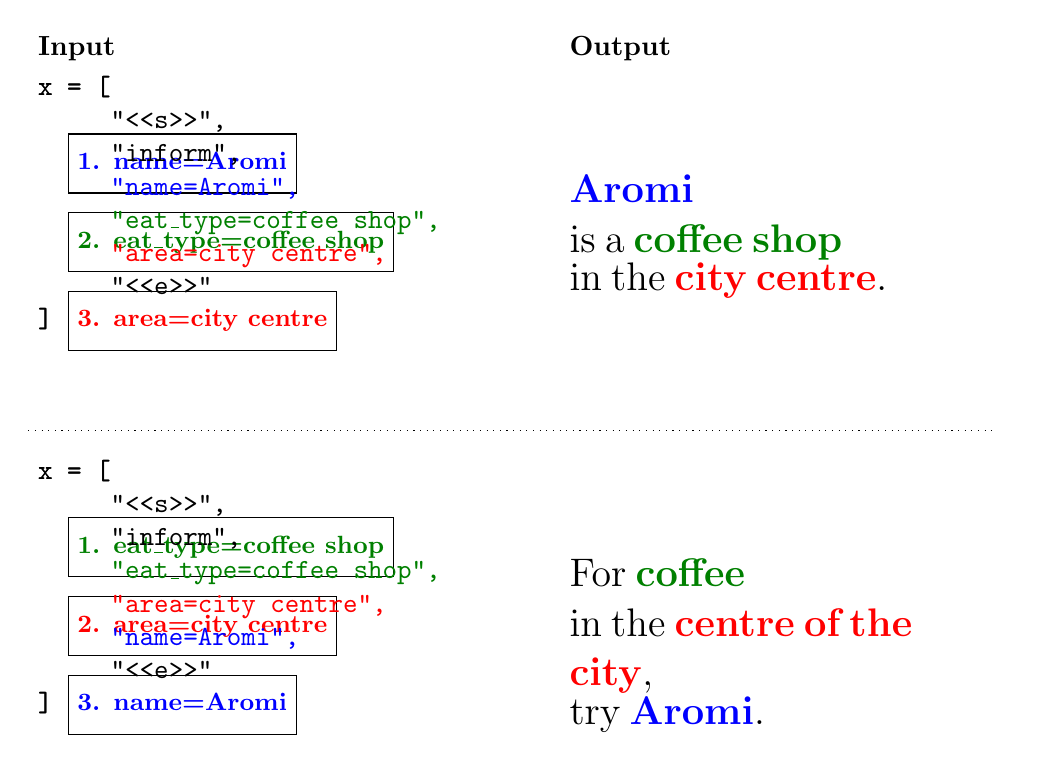
\begin{tikzpicture}[
        plan/.style = {draw,anchor=north west,minimum height=0.75cm,
                       font=\small,text height=0.2cm,text depth=0.05cm},
        plan.name/.style = {plan,text=Blue},
        plan.eat/.style = {plan,text=Green},
        plan.area/.style = {plan,text=Red},
        input/.style = {anchor=north west}]

      \def\plY{3.25};
      \def\plOffset{0.85};
      
      \node[anchor=north west] at (0,3*\plY+0.5) {\textbf{Input}};
      \node[anchor=north west] at (6.75,3*\plY+0.5) {\textbf{Output}};
      \uncover<1>{
        \node[plan.name] at (0.5, 3.0*\plY-\plOffset) {\textbf{1. name=Aromi}};
        \node[plan.eat]  at (0.5, 3.0*\plY-\plOffset-1) {\textbf{2. eat\_type=coffee shop}};
        \node[plan.area] at (0.5, 3.0*\plY-\plOffset-2) {\textbf{3. area=city centre}};
      }

      \draw[dotted] (0,1.5*\plY + 0.25) -- (12.25,1.5*\plY + 0.25);

      \uncover<4>{
        \node[plan.eat]  at (0.5,1.5*\plY-\plOffset) {\textbf{1. eat\_type=coffee shop}};
        \node[plan.area] at (0.5,1.5*\plY-\plOffset-1) {\textbf{2. area=city centre}};
        \node[plan.name] at (0.5,1.5*\plY-\plOffset-2) {\textbf{3. name=Aromi}};
      }


      \uncover<1>{
        \node[input,align=left] at (0.0, 3*\plY) 
        {\texttt{x = [}\\
                \phantom{\texttt{~~~~~"<<s>>",}} \\
                    \phantom{\texttt{~~~~~"inform",}}\\
             \phantom{\texttt{~~~~~"name=Aromi",}}\\
             \phantom{\texttt{~~~~~"eat\_type=coffee shop",}}\\
             \phantom{\texttt{~~~~~"area=city centre",}}\\
             \phantom{\texttt{~~~~~"<<e>>"}}\\
    \texttt{]}};
      }
      \uncover<2->{
        \node[input,align=left] at (0.0, 3*\plY) 
        {\texttt{x = [}\\
         \texttt{~~~~~"<<s>>",} \\
         \texttt{~~~~~"inform",}\\
         \texttt{~~~~~\color{Blue}"name=Aromi",}\\
         \texttt{~~~~~\color{Green}"eat\_type=coffee shop",}\\
         \texttt{~~~~~\color{Red}"area=city centre",}\\
         \texttt{~~~~~"<<e>>"}\\
    \texttt{]}};
      }

      \uncover<4>{
        \node[input,align=left] at (0.0, 1.5*\plY) 
        {\texttt{x = [}\\
                \phantom{\texttt{~~~~~"<<s>>",}} \\
                    \phantom{\texttt{~~~~~"inform",}}\\
             \phantom{\texttt{~~~~~"eat\_type=coffee shop",}}\\
             \phantom{\texttt{~~~~~"area=city centre",}}\\
             \phantom{\texttt{~~~~~"name=Aromi",}}\\
             \phantom{\texttt{~~~~~"<<e>>"}}\\
    \texttt{]}};
      }
      \uncover<5->{
        \node[input,align=left] at (0.0, 1.5*\plY) 
        {\texttt{x = [}\\
         \texttt{~~~~~"<<s>>",} \\
         \texttt{~~~~~"inform",}\\
         \texttt{~~~~~\color{Green}"eat\_type=coffee shop",}\\
         \texttt{~~~~~\color{Red}"area=city centre",}\\
         \texttt{~~~~~\color{Blue}"name=Aromi",}\\
         \texttt{~~~~~"<<e>>"}\\
    \texttt{]}};
      }



      \uncover<3->{
      \node[anchor=north west,text width=5.5cm,align=left] at (6.75,3*\plY-1.25) {\Large {\color{Blue}\uline{\textbf{Aromi}}}\\ is a {\color{Green}\uline{\textbf{coffee shop}}}\\ in the {\color{Red}\uline{\textbf{city centre}}}.};
  }

  \uncover<6>{
  \node[anchor=north west,text width=5.5cm,align=left] at (6.75,1.5*\plY-1.25) {\Large For {\color{Green}\uline{\textbf{coffee}}}\\ in the {\color{Red}\uline{\textbf{centre of the city}}},\\ try {\color{Blue}\uline{\textbf{Aromi}}}.} ;

}

    \end{tikzpicture}
}
        \end{center}

\end{frame}


\begin{frame}{Alignment Training Yields Controllable Generation}

\begin{itemize}
    \item Alignment Training, an input transformation for Seq2Seq to models,
    makes a model controllable at the level of 
    realization ordering.

      \begin{itemize}
        \item<2-> biGRU       follows model-based plans $>89\%$--$100\%$ of the time
        \item<3->  Transformer follows model-based plans $>79\%$--$100\%$ of the time.
        \item<4-> BART (fine-tuned) follows model-based plans $>98\%$--$100\%$ of the time.
       
\end{itemize}

\vspace{10pt}

    \item<5-> We also show that Alignment Training also improves faithfulness
    compared to other linearization strategies. E.g., on E2E challenge test set,
        \begin{itemize}
            \item Transformer with arbitrary linearization gets $0.66\%$--$3.10\%$ Semantic Error Rate
            \item with alignment training gets $0\%$ Semantic Error Rate
        \end{itemize}
      \end{itemize}

\end{frame}

%\begin{frame}{Contributions}
%
%\begin{itemize}
%\item We demonstrate some model limitations as well.
%\begin{itemize}
%\item We perform a random permutation stress test to see how well models 
%perform on difficult plans.
%\end{itemize}
%\end{itemize}
%
%\end{frame}

\pgfplotstableread[row sep=\\,col sep=&]{
    interval        & NUP & Rand & DA \\
    biGRU           & 98.72 & 94.44 & 97.34  \\
    Trans.     & 99.64  & 95.20 & 98.10 \\
    BART            & 96.52 & 97.78 & 98.78 \\
    }\EtoEPermOA

\pgfplotstableread[row sep=\\,col sep=&]{
    interval        & NUP & Rand & DA\\
    biGRU           & 62.04 & 46.72 &  49.26 \\
    Trans.     & 31.34 & 18.70 & 18.10  \\
    BART            & 91.40 & 82.00 & 87.98 \\
    }\ViggoPermOA


\begin{frame}{Random Permutation Stress Test}
\begin{tikzpicture}
    \begin{axis}[
            ybar,
            bar width=.15cm,
            width=0.5\textwidth,
            height=.35\textwidth,
            symbolic x coords={biGRU,Trans.,BART},
            ymajorgrids={true},
            xtick=data,
            %nodes near coords,
            nodes near coords align={vertical},
            enlarge x limits=0.25,
            ymin=90,ymax=100,
            ylabel={Order Acc. (\%)},
            title={E2E},
        ]
        \addplot[fill=Red,color=Red!40,postaction={pattern=dots}] table[x=interval,y=NUP]{\EtoEPermOA};
        \addplot[fill=Blue!20,draw=Blue] table[x=interval,y=Rand]{\EtoEPermOA};
      %\only<2->{  \addplot[fill=Green!20,draw=Green,postaction={
      %  pattern=north east lines,pattern color=Green
    %}] table[x=interval,y=DA]{\EtoEPermOA};}

\only<1>{
\node[xshift=3.0] (a1) at (axis cs:biGRU,98.72) {};
\node[xshift=3.0] (a2) at (axis cs:biGRU,94.44) {};
\node[xshift=3.0] (b1) at (axis cs:Trans.,99.64) {};
\node[xshift=3.0] (b2) at (axis cs:Trans.,95.20) {};
\draw[->,draw=Red,line width=0.5mm] (a1.center) -- (a2.center); 
\draw[->,draw=Red,line width=0.5mm] (b1.center) -- (b2.center); 
}

%\only<2->{
%\node[xshift=0.0] (a1) at (axis cs:biGRU,98.72) {};
%\node[xshift=0.0] (a2) at (axis cs:biGRU,94.44) {};
%\node[xshift=0.0] (b1) at (axis cs:Trans.,99.64) {};
%\node[xshift=0.0] (b2) at (axis cs:Trans.,95.20) {};
%\draw[->,draw=Red,line width=0.5mm] (a1.center) -- (a2.center); 
%\draw[->,draw=Red,line width=0.5mm] (b1.center) -- (b2.center); 
%}


    \end{axis}

    \begin{axis}[
            ybar,
            xshift=6.5cm,
            bar width=.15cm,
            width=0.5\textwidth,
            height=.35\textwidth,
            legend style={at={(0.0,1)}, nodes={scale=0.6, transform shape},
                anchor=north west,legend columns=1},
            symbolic x coords={biGRU,Trans.,BART},
            xtick=data,
            ymajorgrids={true},
            %nodes near coords,
            nodes near coords align={vertical},
            ymin=15,ymax=100,
            enlarge x limits=0.25,
            %ylabel={Order Acc. (\%) },
            title={ViGGO},
        ]
        \addplot[fill=Red,color=Red!40,postaction={pattern=dots}] table[x=interval,y=NUP]{\ViggoPermOA};
        \addplot[fill=Blue!20,draw=Blue] table[x=interval,y=Rand]{\ViggoPermOA};
%       \only<2->{ \addplot[fill=Green!20,draw=Green,postaction={
 %       pattern=north east lines,pattern color=Green
 %   }] table[x=interval,y=DA]{\ViggoPermOA};}
        \legend{NeuralUP,Random,Random+DataAug}

\only<1>{
\node[xshift=3.0] (a1) at (axis cs:biGRU,62.04) {};
\node[xshift=3.0] (a2) at (axis cs:biGRU,46.72) {};
\node[xshift=3.0] (b1) at (axis cs:Trans.,31.64) {};
\node[xshift=3.0] (b2) at (axis cs:Trans.,18.70) {};

\node[xshift=3.0] (c1) at (axis cs:BART,91.40) {};
\node[xshift=3.0] (c2) at (axis cs:BART,82.00) {};
\draw[->,draw=Red,line width=0.5mm] (a1.center) -- (a2.center); 
\draw[->,draw=Red,line width=0.5mm] (b1.center) -- (b2.center); 
\draw[->,draw=Red,line width=0.5mm] (c1.center) -- (c2.center); 
}
%\only<2>{
%\node[xshift=0.0] (a1) at (axis cs:biGRU,62.04) {};
%\node[xshift=0.0] (a2) at (axis cs:biGRU,46.72) {};
%\node[xshift=0.0] (b1) at (axis cs:Trans.,31.64) {};
%\node[xshift=0.0] (b2) at (axis cs:Trans.,18.70) {};
%
%\node[xshift=0.0] (c1) at (axis cs:BART,91.40) {};
%\node[xshift=0.0] (c2) at (axis cs:BART,82.00) {};
%\draw[->,draw=Red,line width=0.5mm] (a1.center) -- (a2.center); 
%\draw[->,draw=Red,line width=0.5mm] (b1.center) -- (b2.center); 
%\draw[->,draw=Red,line width=0.5mm] (c1.center) -- (c2.center); 
%}


    \end{axis}


\uncover<1>{
%\node[draw,fill=white,text width=8.5cm] (a)  at (4.5,-1.5) {\textbf{Alignment Training} Yields Consistent Reductions 
%in Semantic Error over other linearization strategies. };
%
%\draw[line width=0.5mm,->] (a) -- (4.80,0);
%\draw[line width=0.5mm,->] (a) -- (8.65,0);
%\draw[line width=0.5mm,->] (a) -- (1.0,0);
%\draw[line width=0.5mm,->] (a) -- (1.0,-4.8);
%\draw[line width=0.5mm,->] (a) -- (8.65,-4.9);
%\draw[line width=0.5mm,->] (a) -- (4.80,-4.6);
}
\end{tikzpicture}
\begin{itemize} 
\item We demonstrate some model limitations as well.
\begin{itemize}
\item We perform a random permutation stress test to see how well models perform on difficult plans.
    \item Models struggle to realize the same content when it is randomly ordered compared to a plan produced by an Utterance Planner model.
%\item<2-> A phrase-based data augmentation improves the ability to follow difficult plans.
\end{itemize}
\end{itemize}


\end{frame}

\begin{frame}{Phrase-based Data Augmentation}
    \resizebox{\textwidth}{!}{
        \begin{tikzpicture}

            \def\th{5mm};
            \def\td{2mm};
    \node[text height=\th,text depth=\td] (aromi) at (-5,-4) {Aromi};
            \node[text height=\th,text depth=\td] (is) at (-1.5,-4) {is};
            \node[text height=\th,text depth=\td] (not) at (0.0,-4) {not};

            \node[text height=\th,text depth=\td] (a) at (1.5,-4) {a};
            \node[text height=\th,text depth=\td] (ff) at (4,-4) {family-friendly};
            \node[text height=\th,text depth=\td] (est) at (6.5,-4) {establishment};


            \uncover<2->{
            \node (root) at (-2.5,0) {S};
            \node (rootNP) at (-5,-1) {NP};
            \node (rootNPNNP) at (-5,-2) {NNP};
            \only<1-3>{
            \node (r1c2) at (0.0,-1) {VP};
        }
            \only<4->{
                \node[color=mLightBrown] (r1c2) at (0.0,-1) {VP};

            }
            \only<1-2>{
                \node (r2c3) at (4,-2) {NP};
                \node (det) at (1.5,-3) {DET};
                \node (jj) at (4,-3) {JJ};
                \node (nn) at (6.5,-3) {NN};
            }
            \only<3->{
                \node[color=mLightBrown] (r2c3) at (4,-2) {NP};
                \node[color=mLightBrown] (det) at (1.5,-3) {DET};
                \node[color=mLightBrown] (jj) at (4,-3) {JJ};
                \node[color=mLightBrown] (nn) at (6.5,-3) {NN};
            }
            \only<1-3>{
                \node (r2c1) at (-1.5,-2) {VB};
                \node (r2c2) at (0.0,-2) {RB};
                \draw[-] (r1c2) -- (r2c1);
                \draw[-] (r1c2) -- (r2c2);
                \draw[-] (r1c2) -- (r2c3);
            }
            \only<4->{
                \node[color=mLightBrown] (r2c1) at (-1.5,-2) {VB};
                \node[color=mLightBrown] (r2c2) at (0.0,-2) {RB};
                \draw[mLightBrown,-] (r1c2) -- (r2c1);
                \draw[mLightBrown,-] (r1c2) -- (r2c2);
                \draw[mLightBrown,-] (r1c2) -- (r2c3);
            }


            \only<1-3>{
                \draw[-] (r2c1) -- (is);
            }
            \only<4->{
                \draw[color=mLightBrown,-] (r2c1) -- (is);

            }
            \draw[-] (rootNPNNP) -- (aromi);
            \draw[-] (root.south west) -- (rootNP.north east);
            \draw[-] (rootNP) -- (rootNPNNP);
            \draw[-] (root.south east) -- (r1c2.north west);
            \only<1-2>{
                \draw[-] (r2c3) -- (det);
                \draw[-] (r2c3) -- (jj);
                \draw[-] (r2c3) -- (nn);
                \draw[-] (det) -- (a);
                \draw[-] (jj) -- (ff);
                \draw[-] (nn) -- (est);
            }
            \only<3->{
                \draw[mLightBrown,-] (r2c3) -- (det);
                \draw[mLightBrown,-,color=mLightBrown] (r2c3) -- (jj);
                \draw[mLightBrown,-,color=mLightBrown] (r2c3) -- (nn);
                \draw[mLightBrown,-] (det) -- (a);
                \draw[mLightBrown,-] (jj) -- (ff);
                \draw[mLightBrown,-] (nn) -- (est);
            }
            \only<1-3>{
                \draw[-] (r2c2) -- (not);
            }
            \only<4>{
                \draw[color=mLightBrown,-] (r2c2) -- (not);
            }
        }
        

            \node[anchor=north west,align=left,inner sep=0,outer sep=0,text height=0mm,text width=11cm] at (0.7,0.5) {
                    \begin{enumerate}
                        \item<2-> Parse training examples.
                \item<3-> Create additional training examples from constituent phrases.
                \end{enumerate}};

        \end{tikzpicture}
    }

    \uncover<3->{
    \resizebox{\textwidth}{!}{
        {  \begin{minipage}{1.45\textwidth}
$\left[\!\!\!\left[\begin{array}{l} \textsc{Inform} \\ \textrm{family\_friendly=yes} \end{array} \right]\!\!\!\right]$ \texttt{["a", "family-friendly", "establishment"]}
\end{minipage}}}
}
\uncover<4>{
    \resizebox{\textwidth}{!}{
        {  \begin{minipage}{1.45\textwidth}
$\left[\!\!\!\left[\begin{array}{l} \textsc{Inform} \\  \textrm{family\_friendly=no} \end{array} \right]\!\!\!\right]$ \texttt{["is", "not", "a", "family-friendly", "establishment"]}
\end{minipage}}}}


\end{frame}

\begin{frame}{Random Permutation Stress Test}
\begin{tikzpicture}
    \begin{axis}[
            ybar,
            bar width=.15cm,
            width=0.5\textwidth,
            height=.35\textwidth,
            symbolic x coords={biGRU,Trans.,BART},
            ymajorgrids={true},
            xtick=data,
            %nodes near coords,
            nodes near coords align={vertical},
            enlarge x limits=0.25,
            ymin=90,ymax=100,
            ylabel={Order Acc. (\%)},
            title={E2E},
        ]
        \addplot[fill=Red,color=Red!40,postaction={pattern=dots}] table[x=interval,y=NUP]{\EtoEPermOA};
        \addplot[fill=Blue!20,draw=Blue] table[x=interval,y=Rand]{\EtoEPermOA};
      \only<2->{  \addplot[fill=Green!20,draw=Green,postaction={
        pattern=north east lines,pattern color=Green
    }] table[x=interval,y=DA]{\EtoEPermOA};}

\only<1>{
\node[xshift=3.0] (a1) at (axis cs:biGRU,98.72) {};
\node[xshift=3.0] (a2) at (axis cs:biGRU,94.44) {};
\node[xshift=3.0] (b1) at (axis cs:Trans.,99.64) {};
\node[xshift=3.0] (b2) at (axis cs:Trans.,95.20) {};
\draw[->,draw=Red,line width=0.5mm] (a1.center) -- (a2.center); 
\draw[->,draw=Red,line width=0.5mm] (b1.center) -- (b2.center); 
}

\only<2->{
\node[xshift=0.0] (a1) at (axis cs:biGRU,98.72) {};
\node[xshift=0.0] (a2) at (axis cs:biGRU,94.44) {};
\node[xshift=0.0] (b1) at (axis cs:Trans.,99.64) {};
\node[xshift=0.0] (b2) at (axis cs:Trans.,95.20) {};
\draw[->,draw=Red,line width=0.5mm] (a1.center) -- (a2.center); 
\draw[->,draw=Red,line width=0.5mm] (b1.center) -- (b2.center); 
}


    \end{axis}

    \begin{axis}[
            ybar,
            xshift=6.5cm,
            bar width=.15cm,
            width=0.5\textwidth,
            height=.35\textwidth,
            legend style={at={(0.0,1)}, nodes={scale=0.6, transform shape},
                anchor=north west,legend columns=1},
            symbolic x coords={biGRU,Trans.,BART},
            xtick=data,
            ymajorgrids={true},
            %nodes near coords,
            nodes near coords align={vertical},
            ymin=15,ymax=100,
            enlarge x limits=0.25,
            %ylabel={Order Acc. (\%) },
            title={ViGGO},
        ]
        \addplot[fill=Red,color=Red!40,postaction={pattern=dots}] table[x=interval,y=NUP]{\ViggoPermOA};
        \addplot[fill=Blue!20,draw=Blue] table[x=interval,y=Rand]{\ViggoPermOA};
       \only<2->{ \addplot[fill=Green!20,draw=Green,postaction={
        pattern=north east lines,pattern color=Green
    }] table[x=interval,y=DA]{\ViggoPermOA};}
        \legend{NeuralUP,Random,Random+DataAug}

\only<1>{
\node[xshift=3.0] (a1) at (axis cs:biGRU,62.04) {};
\node[xshift=3.0] (a2) at (axis cs:biGRU,46.72) {};
\node[xshift=3.0] (b1) at (axis cs:Trans.,31.64) {};
\node[xshift=3.0] (b2) at (axis cs:Trans.,18.70) {};

\node[xshift=3.0] (c1) at (axis cs:BART,91.40) {};
\node[xshift=3.0] (c2) at (axis cs:BART,82.00) {};
\draw[->,draw=Red,line width=0.5mm] (a1.center) -- (a2.center); 
\draw[->,draw=Red,line width=0.5mm] (b1.center) -- (b2.center); 
\draw[->,draw=Red,line width=0.5mm] (c1.center) -- (c2.center); 
}
\only<2>{
\node[xshift=0.0] (a1) at (axis cs:biGRU,62.04) {};
\node[xshift=0.0] (a2) at (axis cs:biGRU,46.72) {};
\node[xshift=0.0] (b1) at (axis cs:Trans.,31.64) {};
\node[xshift=0.0] (b2) at (axis cs:Trans.,18.70) {};

\node[xshift=0.0] (c1) at (axis cs:BART,91.40) {};
\node[xshift=0.0] (c2) at (axis cs:BART,82.00) {};
\draw[->,draw=Red,line width=0.5mm] (a1.center) -- (a2.center); 
\draw[->,draw=Red,line width=0.5mm] (b1.center) -- (b2.center); 
\draw[->,draw=Red,line width=0.5mm] (c1.center) -- (c2.center); 
}


    \end{axis}


\end{tikzpicture}
\begin{itemize} 
\item We demonstrate some model limitations as well.
\begin{itemize}
\item We perform a random permutation stress test to see how well models perform on difficult plans.
    \item Models struggle to realize the same content when it is randomly ordered compared to a plan produced by an Utterance Planner model.
%\item<2-> A phrase-based data augmentation improves the ability to follow difficult plans.
\end{itemize}
\end{itemize}


\end{frame}


\begin{frame}{Contributions}


\begin{itemize}



    \item We introduce an input transformation for Seq2Seq to models
    called Alignment Training that makes a model controllable at the level
    realization ordering.

\vspace{10pt}

    \item We  show that Alignment Training also improves faithfulness
    compared to other linearization strategies. 

\vspace{10pt}
\item We perform a random permutation stress test to see how well models perform on difficult plans, and show that performance degrades in this setting.

\vspace{10pt}
\item We propose a phrase based data augmentation method which improves 
performance in this more difficult setting.

\end{itemize}

\end{frame}


